\documentclass[english]{article}
\usepackage[T1]{fontenc}
\usepackage[latin9]{inputenc}
\usepackage{babel}
\usepackage{graphicx}
\usepackage{subfigure}
\usepackage{float}
\setlength{\parindent}{0pt}

\begin{document}

\title{Lab 1: Polarization Imaging\\ -------------------------------- \\ \Large Sensors and Digitization}
\author{ \ Armine Vardazaryan, Songyou Peng \\ arminevardazaryan@gmail.com, psy920710@gmail.com}
\date{18th November 2015}

\maketitle

\section{Introduction}

\section{Simplified polarization imaging}
Firstly, in order to answer the fifth question in the "\textbf{Getting started}" part, we rotate the polarizer from 0\textdegree to 90\textdegree. The result can be seen in the figure \ref{fig:one}. Please notice the cellphone screen in the pictures. When the angle of polarizer is 0\textdegree, the screen has a really high intensity, with the 90\textdegree one an extremely low intensity. Due to that, we are able to say that this cellphone are polarized in the direction of 0\textdegree.\\

\begin{figure}[H]
	\centering
	\subfigure[0\textdegree]{\label{fig:onea}
	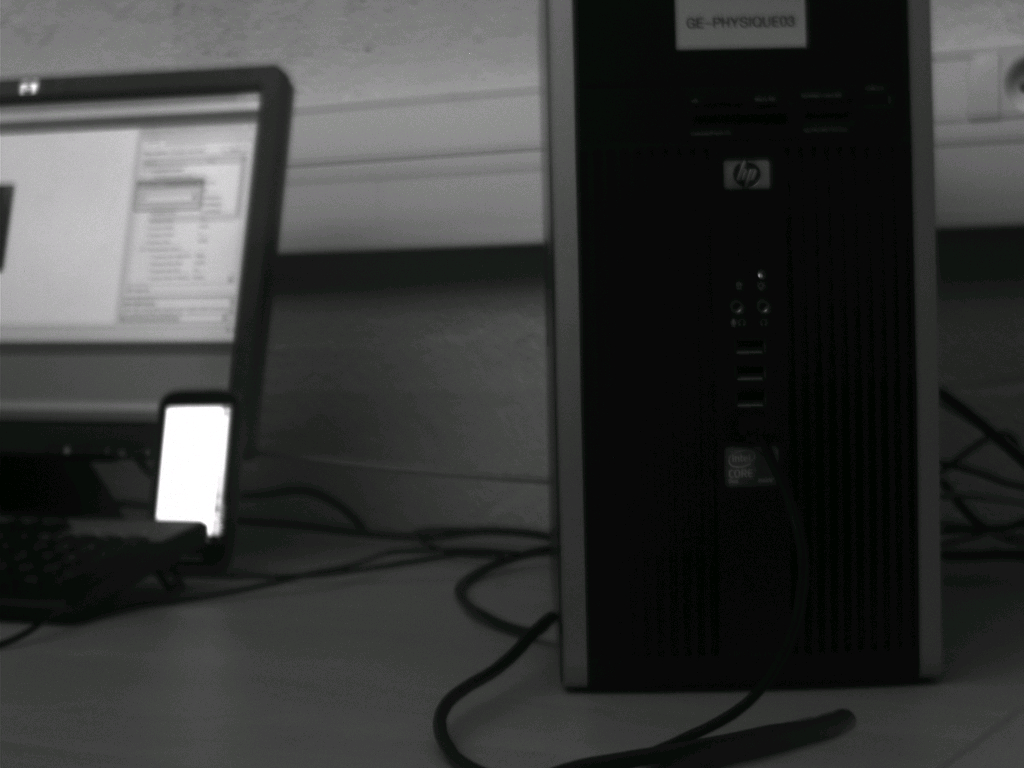
\includegraphics[width=0.3\linewidth]{Pictures/wolff/0.jpg}
	}
	\subfigure[45\textdegree]{\label{fig:oneb}
	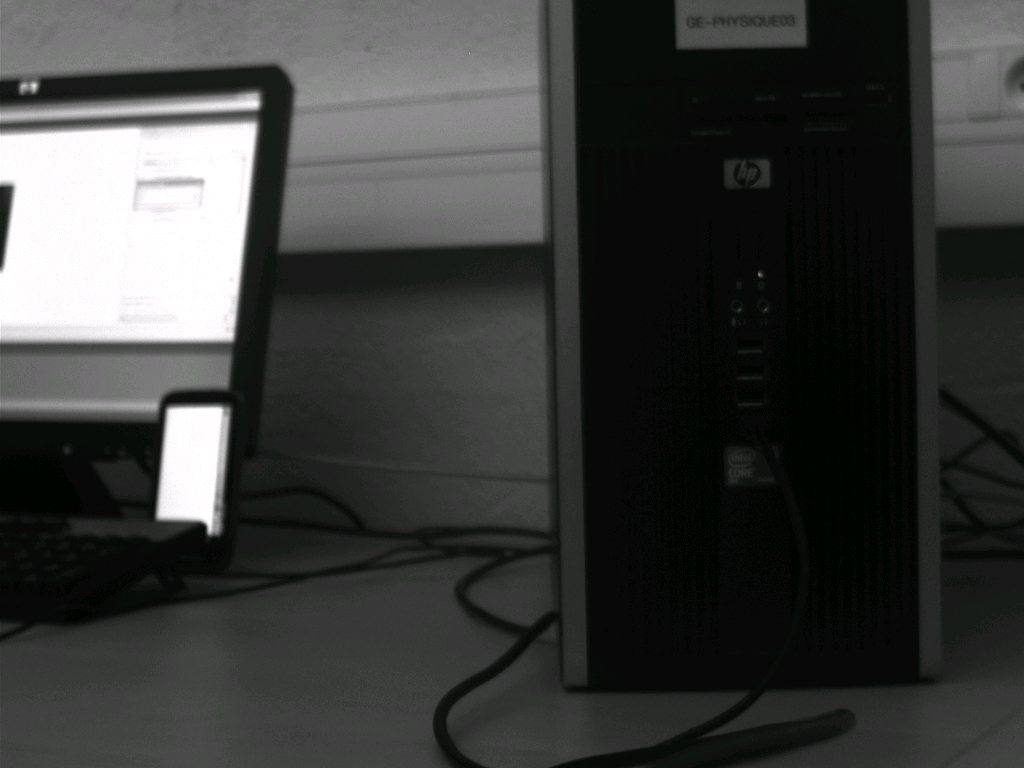
\includegraphics[width=0.3\linewidth]{Pictures/wolff/45.jpg}
	}
	\subfigure[90\textdegree]{\label{fig:onethree}
	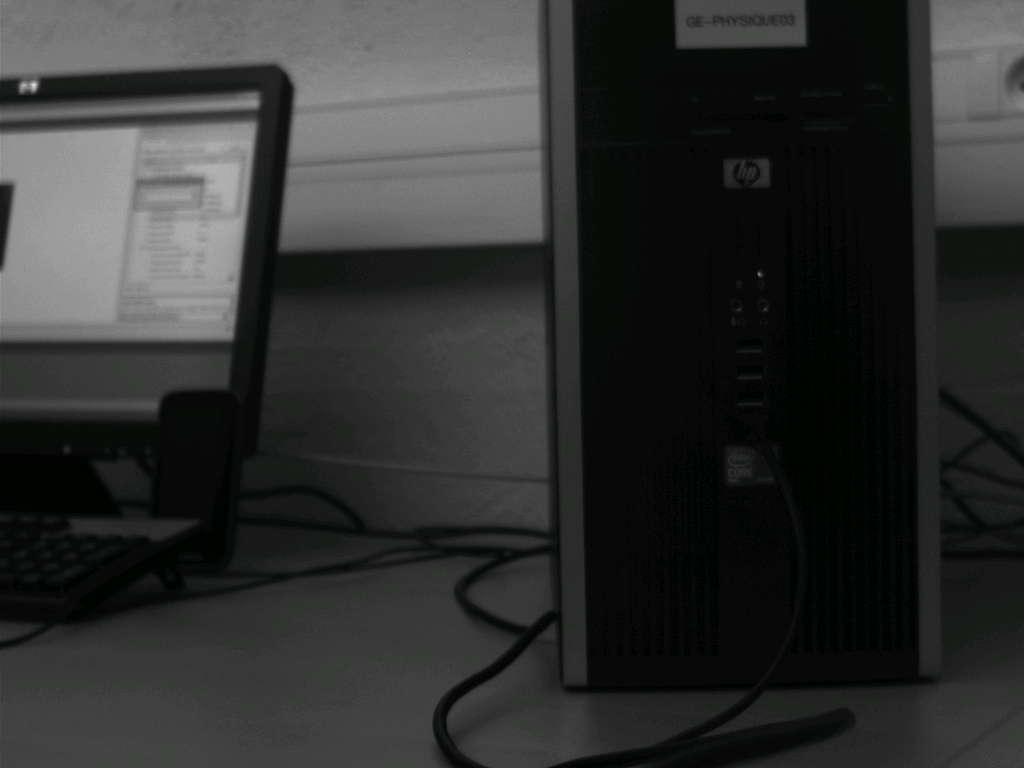
\includegraphics[width=0.3\linewidth]{Pictures/wolff/90.jpg}
	}
	\caption{Pictures in different angles of polarizer}
	\label{fig:one}
\end{figure}

\subsection{Wolff's method}
Before taking any pictures, we set the autoexposure and gain of the camera to be manual because we want to keep everything of camera the same, so that we can eliminate any effect from camera itself.\\
\\
After taking pictures with the polarizer orientation: 0\textdegree, 45\textdegree, 90\textdegree, we first compute the total light intensity $I$ based on the equation:
$$
I = I_{0} + I_{90}
$$

\subsection{Least Mean Square method}

\section{Contrast polarization measurement}

\subsection{Polarisers and a rotator}
First, we set up the system with two polarisers, both oriented to $0\deg$. <pictures>\\
We see that the intensity of the light decreases with adding each polariser. After the first polariser, the light is dimmed because the light is randomly oriented and according to Malus's law the light is, in fact, halved:\\
\\
$I=\frac{1}{2\pi}\int_0^{2\pi}I_{o}\cos(\theta)^2\,d\theta=I_{o}/2$\\
\\
After the first polariser, the light is linearly polarised, and again, according to Malus's Law it is diminished according to the following formula:\\
$I=I_ocos^2(θ)$\\
From there we can conclude, that if the angle of polarisation $\Theta$ is $0\deg$, the intensity remains the same as after the first polariser: 1 / 2. But when $\Theta$ is increased, the intensity decreases as well.\\
After that the switchable polarization rotator is inserted between two polarisers. This rotator has only two states: rotate light by $90\deg$ or $0\deg$. So when the polarisers are set to $0\deg$ each and the rotator is on, the light is rotated by $90\deg$, making it perpendicular to the second polariser. That, as we know results in total extinguishing of any light passing. However when the rotator is off, no difference is noticeable.\\
\begin{figure}[H]
	\centering
	\subfigure[0\textdegree]{\label{fig:rotatorzero}
	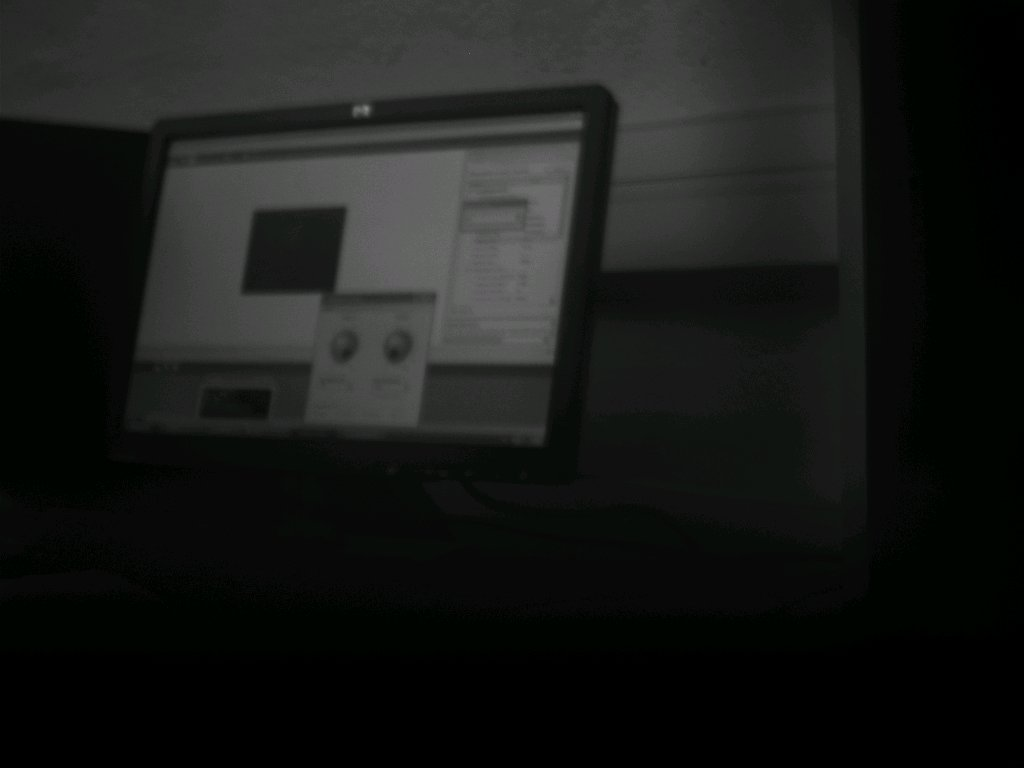
\includegraphics[width=0.3\linewidth]{Pictures/retarder/0.jpg}
	}
	\subfigure[90\textdegree]{\label{fig:rotatorninety}
	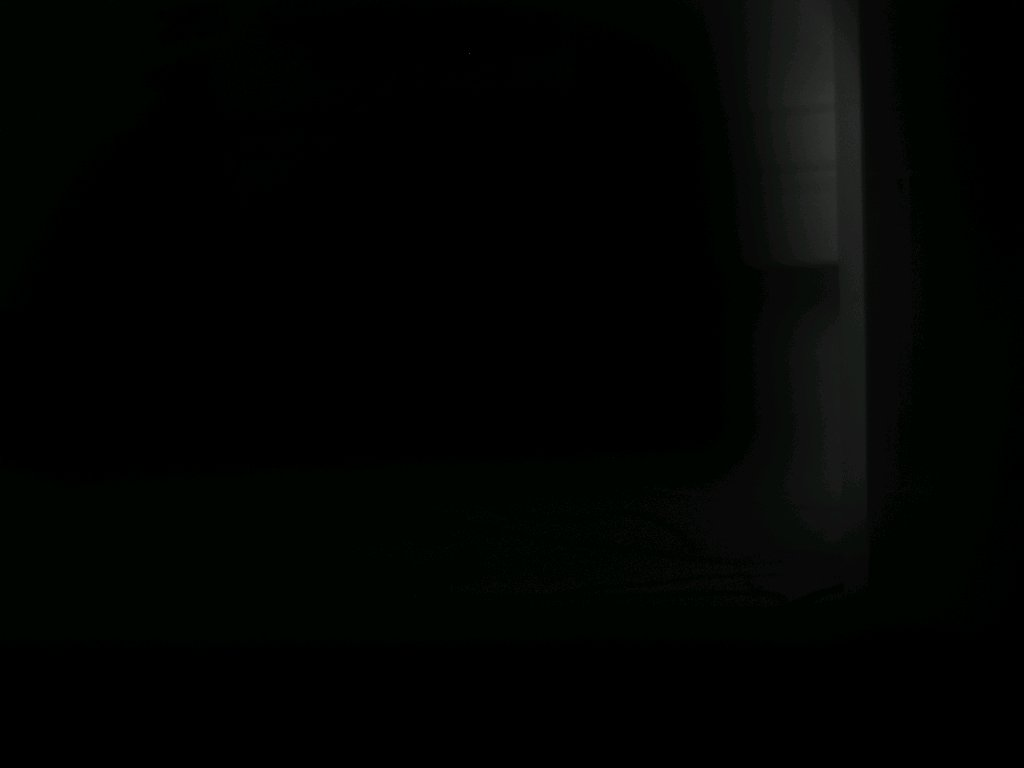
\includegraphics[width=0.3\linewidth]{Pictures/retarder/90.jpg}
	}
	\caption{Polariser with a rotator(off in the first image, and on in the second)}
	\label{fig:one}
\end{figure}
\subsection{Diffused and specular reflection}
In this section we experiment with diffused and specular reflections, and how the polariser affects that kind of light.\\
Specular reflection can be seen when light is reflected from smooth surfaces and the reflected light becomes polarised. Diffused reflection is caused when light falls onto a rough surface. The reflected light is not polarised but diffused in this case.\\
To test that, we introduced a polarised light source into the system, before the rotator. \\
We observe that the glare of light is mostly removed from the shiny surface, while the intensity is only dimmed for the diffused reflection.
\begin{figure}[H]
	\centering
	\subfigure[90\textdegree]{\label{fig:rotatorzero}
	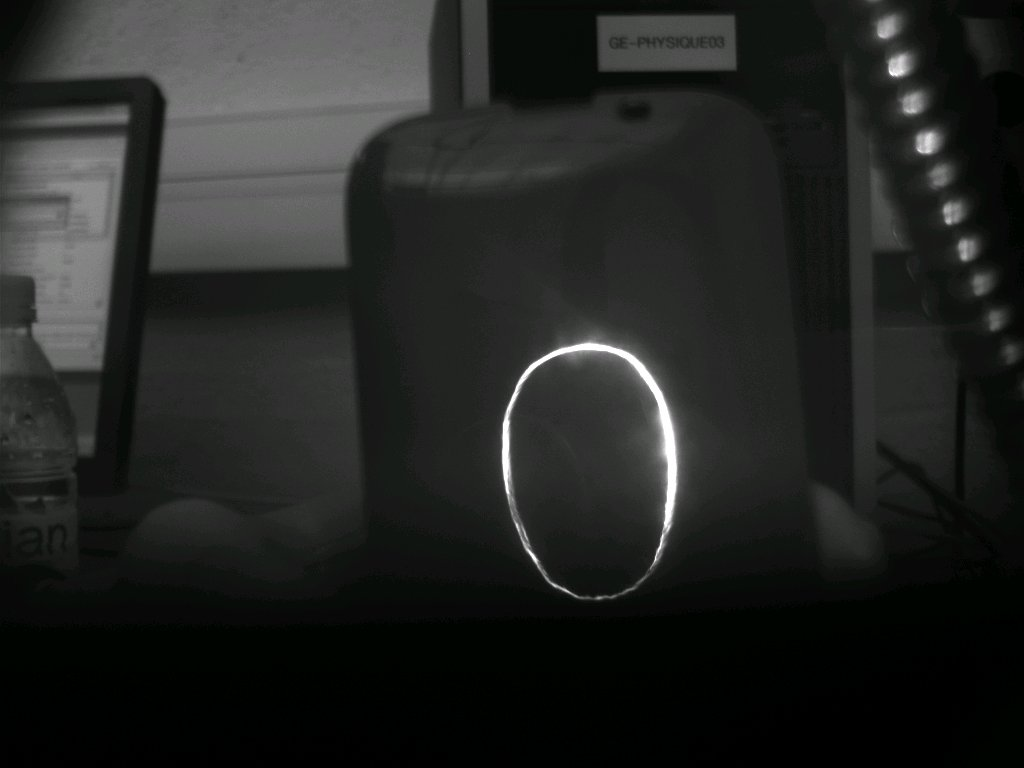
\includegraphics[width=0.3\linewidth]{Pictures/reflect/90.jpg}
	}
	\subfigure[90\textdegree]{\label{fig:rotatorninety}
	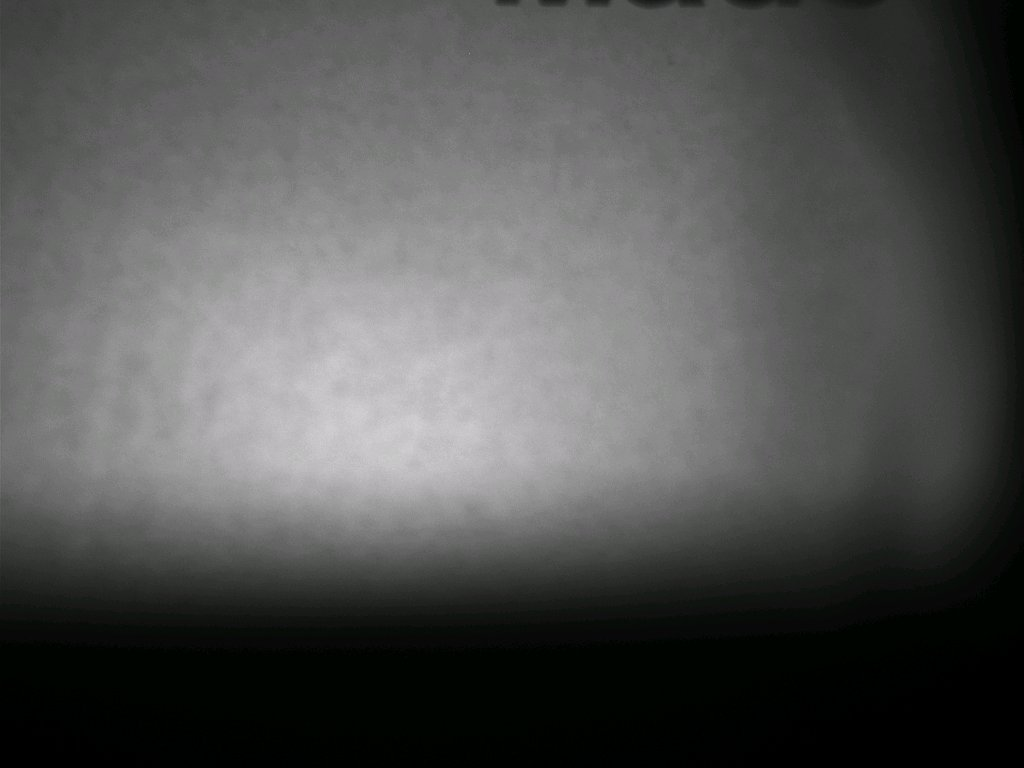
\includegraphics[width=0.3\linewidth]{Pictures/reflect/d90.jpg}
	}
	\caption{Specular and diffused reflection with polariser}
	\label{fig:one}
\end{figure}

\section{Conclusion}

\section{References}

{[}1{]} -http://www.measurecentral.com

\end{document}